\documentclass[12pt]{scrartcl}

\setlength{\parindent}{0pt}
\setlength{\parskip}{.25cm}

\usepackage{graphicx}

\usepackage{xcolor}

\definecolor{darkred}{rgb}{0.5,0,0}
\definecolor{darkgreen}{rgb}{0,0.5,0}
\usepackage{hyperref}
\hypersetup{
  letterpaper,
  colorlinks,
  linkcolor=red,
  citecolor=darkgreen,
  menucolor=darkred,
  urlcolor=blue,
  pdfpagemode=none,
  pdftitle={CSCE 156 Lab Handout},
  pdfauthor={Christopher M. Bourke},
  pdfsubject={},
  pdfkeywords={}
}

\definecolor{MyDarkBlue}{rgb}{0,0.08,0.45}
\definecolor{MyDarkRed}{rgb}{0.45,0.08,0}
\definecolor{MyDarkGreen}{rgb}{0.08,0.45,0.08}

\definecolor{mintedBackground}{rgb}{0.95,0.95,0.95}
\definecolor{mintedInlineBackground}{rgb}{.90,.90,1}

%\usepackage{newfloat}
\usepackage[newfloat=true]{minted}
\setminted{mathescape,
               linenos,
               autogobble,
               frame=none,
               framesep=2mm,
               framerule=0.4pt,
               %label=foo,
               xleftmargin=2em,
               xrightmargin=0em,
               startinline=true,  %PHP only, allow it to omit the PHP Tags *** with this option, variables using dollar sign in comments are treated as latex math
               numbersep=10pt, %gap between line numbers and start of line
               style=default, %syntax highlighting style, default is "default"
               			    %gallery: http://help.farbox.com/pygments.html
			    	    %list available: pygmentize -L styles
               bgcolor=mintedBackground} %prevents breaking across pages
               
\setmintedinline{bgcolor={mintedBackground}}
\setminted[text]{bgcolor={mintedBackground},linenos=false,autogobble,xleftmargin=1em}
%\setminted[php]{bgcolor=mintedBackgroundPHP} %startinline=True}
\SetupFloatingEnvironment{listing}{name=Code Sample}
\SetupFloatingEnvironment{listing}{listname=List of Code Samples}

\title{CSCE 156 -- Computer Science II}
\subtitle{Lab 5.0 - Inheritance}
\author{~}
\date{~}

\begin{document}

\maketitle

\section*{Prior to Lab}

\begin{enumerate}
  \item Review this laboratory handout prior to lab.
  \item Read the following tutorial on inheritance in Java\\
	\url{http://download.oracle.com/javase/tutorial/java/IandI/subclasses.html} 
  \item Read about abstract methods and abstract classes in Java \\
	\url{http://download.oracle.com/javase/tutorial/java/IandI/abstract.html}
  \item Read about interfaces in Java: \\
	\url{http://download.oracle.com/javase/tutorial/java/IandI/createinterface.html}
\end{enumerate}

\section*{Lab Objectives \& Topics}
Following the lab, you should be able to:
\begin{itemize}
  \item Understand Inheritance and design classes and subclasses in Java
  \item Understand and use interfaces and abstract classes in Java
  \item Understand and use the \mintinline{java}{implements} and 
  	\mintinline{java}{extends} keywords
\end{itemize}


\section*{Peer Programming Pair-Up}

To encourage collaboration and a team environment, labs will be
structured in a \emph{pair programming} setup.  At the start of
each lab, you will be randomly paired up with another student 
(conflicts such as absences will be dealt with by the lab instructor).
One of you will be designated the \emph{driver} and the other
the \emph{navigator}.  

The navigator will be responsible for reading the instructions and
telling the driver what to do next.  The driver will be in charge of the
keyboard and workstation.  Both driver and navigator are responsible
for suggesting fixes and solutions together.  Neither the navigator
nor the driver is ``in charge.''  Beyond your immediate pairing, you
are encouraged to help and interact and with other pairs in the lab.

Each week you should alternate: if you were a driver last week, 
be a navigator next, etc.  Resolve any issues (you were both drivers
last week) within your pair.  Ask the lab instructor to resolve issues
only when you cannot come to a consensus.  

Because of the peer programming setup of labs, it is absolutely 
essential that you complete any pre-lab activities and familiarize
yourself with the handouts prior to coming to lab.  Failure to do
so will negatively impact your ability to collaborate and work with 
others which may mean that you will not be able to complete the
lab.  

\section*{Getting Started}

Clone the project code for this lab from GitHub in Eclipse using the
URL, \url{https://github.com/cbourke/CSCE156-Lab05}.
Refer to Lab 1.0 for instructions on how to clone a project from GitHub.

\section*{Inheritance}

Object Oriented Programming allows you to define a hierarchy of objects 
using \emph{inheritance}.  Inheritance promotes code reuse and semantic 
relations between objects.  Subclasses provide specialization of behavior 
by allowing you to override object methods while preserving common 
functionality (generalization) defined in the super-class.

As a class-based object-oriented programming language, Java facilitates 
inheritance through subclassing by using the keyword extends.  If class 
$B$ \mintinline{java}{extend}s class $A$, $B$ is said to be a subclass 
of $A$ ($A$ is a superclass of $B$).  Instances of class $B$ are also 
instances of class $A$, defining an ``is-a'' relation between them. 
Java also provides two related mechanisms related to subclassing.
\begin{itemize}
  \item \emph{Abstract Classes} -- Java allows you to specify that a 
    class is abstract using the keyword \mintinline{java}{abstract}.  
    In an abstract class, you can define not only normal methods (which 
    you provide a ``default'' implementation for) but you can also 
    define abstract methods: methods that you do not need to provide 
    an implementation for.  Instead, it is the responsibility of 
    non-abstract subclass(es) to provide an implementation.  In addition, 
    if a class is abstract, you are prevented from instantiating any 
    instances of it.
  \item \emph{Interfaces} -- Java allows you to define interfaces, 
    which are essentially pure abstract classes.  Interfaces specify 
    the methods that a class must provide in order to implement the 
    interface.  Java allows you to define an interface that specifies 
    the public interface (methods) of a class.  Classes can then be 
    defined to implement an interface using the \mintinline{java}{implements} 
    keyword.  One major advantage of interfaces is that it does not 
    lock your classes into a rigid hierarchy; however objects that 
    implement an interface can still be considered to have the is-a 
    relationship.  In addition, interfaces can be used to simulate 
    multiple-inheritance in Java as classes can implement more than 
    one interface. 
\end{itemize}
    
\section*{Activities}

You will explore these concepts by completing a Java program that 
simulates a basic weekly payroll reporting system for the Cinco 
Corporation.  Every employee has an employee ID, a name (first and 
last), and a title.  Further, there are two types of employees:
\begin{itemize}
  \item Salaried employees -- Salaried employees have a base annual 
  salary, which is subject to a 20\% income tax rate (state, federal 
  and FICA combined).  In addition, each salaried employee receives 
  a \$100 post-tax benefits allowance.
  \item Hourly employees -- Hourly employees have a per-hour pay rate 
  along with a weekly total of the number of hours they worked.  
  Hourly employees do not receive any benefit allowance.  Further, 
  there are two types of hourly employees.
  \begin{itemize}
    \item Staff employees are directly employed by Cinco and are subject 
    to a 15\% income tax rate.
    \item Temporary employees are not directly employed by Cinco, but 
    instead are contracted through a third-party temp agency who is 
    responsible for collecting taxes (thus no taxes are taken from 
    their gross pay).
  \end{itemize}
\end{itemize}
  
Employee data is stored in a flat data file and the basic parsing has 
been provided.  However, you will need to design and implement Java 
classes to support and model this payroll system.  By the end of this
lab your class designs should resemble something like that in Figure
\ref{figure:uml}.

\begin{figure}[h]
\centering
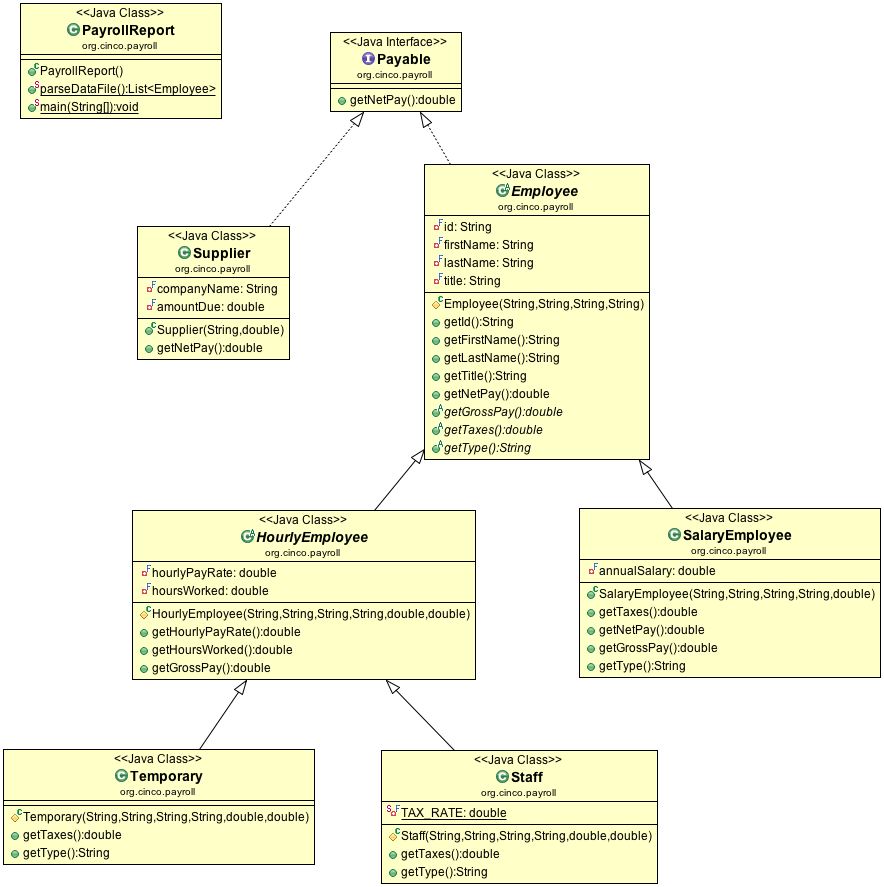
\includegraphics[scale=.40]{ProjectUML}
\caption{UML Diagram of a potential design for the Cinco Corporation 
payroll system}
\label{figure:uml}
\end{figure}

\subsection*{Class Design \& Inheritance}

You have been provided a partially completed 
\mintinline{java}{PayrollReport} program that parses a data file 
(in \mintinline{text}{data/employee.dat}) and creates instances of an 
\mintinline{java}{Employee}.  However, the \mintinline{java}{Employee} 
class is empty.  You will need to implement this class and any relevant 
subclass(es) to complete the program.  
\begin{itemize}
  \item Identify the different classes necessary to model each of the 
    different types of employees in the problem statement.
  \item Identify the relationship between these classes.
  \item Identify the state (variables) that are common to these classes 
    and the state that distinguishes them.  Where do each of these 
    pieces of data belong?
  \item Identify the behavior (methods) that are common to each of 
    these classes--what are methods that should be in the superclass?  
    How should subclasses provide specialized behavior?
  \item Some state/behavior may be common to several classes--is there 
    an opportunity to define an intermediate class?
  \item If you need more guidance, consult the UML diagram below on 
    one possible design.
  \item To check your work, a text file containing the expected output 
    has been provided in the project (see 
    \mintinline{text}{output/expectedOutput.txt})
\end{itemize}

Eclipse Tip: Many of the common programming tasks when dealing with 
objects can be automated by your IDE.  For example: once you have 
designed the state (variables) of your class, you can automatically 
generate the boilerplate getters, setters, and constructors: when 
focused on your class, click ``Source'' $\rightarrow$ ``Generate Getters 
and Setters'' or ``Generate Constructors using Fields.''

Java Note: In a subclass, you \emph{must} invoke a constructor in 
the superclass and it must be done first.  This rule is so that 
classes conform to the is-a relationship.  Invoking a super class's 
constructor is achieved by using the \mintinline{java}{super} keyword.  
If there are multiple constructors, you may invoke any one of them.  
Note that if a constructor does not explicitly invoke a superclass 
constructor, the Java compiler automatically inserts a call to the 
no-argument constructor of the superclass. If the superclass does 
not have a no-argument constructor, you will get a compile-time 
error.  The Java \mintinline{java}{Object} class has a no-arg 
constructor, so if your class does not explicitly extend a class, 
it implicitly \mintinline{java}{extends Object} and the no-arg
constructor is invoked.

\subsection*{Abstractions}

Now that you have a well designed, functional implementation we will 
improve on the design by identifying potential abstractions that can 
be made.  In particular, start by making the \mintinline{java}{Employee} 
class abstract.  If you had a good design, then nothing should break; 
the model did not have any generic employee--all employees were of a 
specific type.  If something did break in your code, rethink your 
design and make the appropriate changes.

Further, identify one or more methods in the \mintinline{java}{Employee} 
class that could be made abstract.  That is, are there any methods in 
the superclass where it would not be appropriate to have a ``default'' 
definition?  Make these methods abstract and again make any appropriate 
changes to your design as necessary.

\subsection*{Adding an Interface}

Cinco Corporation also has suppliers that they purchase supplies 
and parts from to build their products.  Suppliers have a company 
name and an amount due, and so need to be paid, but they are not 
employees.  However, the payroll department would like to have a 
common interface across all objects in their system that are, in 
some way, payable.  

\begin{enumerate}
  \item Create an interface (In Eclipse: right click the package 
    $\rightarrow$ new $\rightarrow$ Interface) called 
    \mintinline{java}{Payable}.  Identify a single method in this 
    interface that returns the (net) amount payable
  \item Make the \mintinline{java}{Employee} class implement this 
    new interface and make the appropriate changes if necessary
  \item Create a new class to represent suppliers and also make it 
    \mintinline{java}{Payable}
  \item Answer the questions in your worksheet
\end{enumerate}

\section*{Advanced Activities (Optional)}

\begin{enumerate}
  \item The \mintinline{java}{PayrollReport} class uses an 
    \mintinline{java}{ArrayList} to hold instances of 
    \mintinline{java}{Employee} objects.  When it generates the report, 
    it does so in the order that the instances were parsed from the 
    data file.  Change this so that the payroll report prints in order 
    of the total net pay in decreasing order.  
    
  \item Unified Modeling Language (UML) is a common tool in Software
    Engineering that provides a visualization of the relationships 
    between software components (subsystems, components, classes, 
    workflows, use cases, etc.).  Sometimes design of systems is done 
    in UML and then tools can automatically generate Java (or other 
    language) code conforming to the design.  Conversely, UML diagrams 
    (like that in Figure \ref{figure:uml}) can be automatically generated 
    from an existing code base using various tools.  In this exercise 
    you will familiarize yourself with UML and use such a tool to 
    generate a UML diagram for your design.
    \begin{itemize}
      \item Read the following tutorial on using UML for class diagrams:
\url{http://www.ibm.com/developerworks/rational/library/content/RationalEdge/sep04/bell/}
      \item Install an Eclipse plugin for UML and generate a UML diagram 
      for your project.  The choice is yours, but one (free) possibility 
      is ObjectAid UML:
      \begin{itemize}
        \item Installation instructions: 
        \url{https://www.objectaid.com/install-objectaid}
	    \item Generate class diagram instructions: 
        \url{http://www.objectaid.com/class-diagram}
      \end{itemize}
    \end{itemize}
\end{enumerate}

\end{document}
